\documentclass[]{article}
\usepackage{lmodern}
\usepackage{amssymb,amsmath}
\usepackage{ifxetex,ifluatex}
\usepackage{fixltx2e} % provides \textsubscript
\ifnum 0\ifxetex 1\fi\ifluatex 1\fi=0 % if pdftex
  \usepackage[T1]{fontenc}
  \usepackage[utf8]{inputenc}
\else % if luatex or xelatex
  \ifxetex
    \usepackage{mathspec}
  \else
    \usepackage{fontspec}
  \fi
  \defaultfontfeatures{Ligatures=TeX,Scale=MatchLowercase}
\fi
% use upquote if available, for straight quotes in verbatim environments
\IfFileExists{upquote.sty}{\usepackage{upquote}}{}
% use microtype if available
\IfFileExists{microtype.sty}{%
\usepackage{microtype}
\UseMicrotypeSet[protrusion]{basicmath} % disable protrusion for tt fonts
}{}
\usepackage[margin=1in]{geometry}
\usepackage{hyperref}
\hypersetup{unicode=true,
            pdftitle={Class05\_R.R},
            pdfauthor={wuzhu},
            pdfborder={0 0 0},
            breaklinks=true}
\urlstyle{same}  % don't use monospace font for urls
\usepackage{color}
\usepackage{fancyvrb}
\newcommand{\VerbBar}{|}
\newcommand{\VERB}{\Verb[commandchars=\\\{\}]}
\DefineVerbatimEnvironment{Highlighting}{Verbatim}{commandchars=\\\{\}}
% Add ',fontsize=\small' for more characters per line
\usepackage{framed}
\definecolor{shadecolor}{RGB}{248,248,248}
\newenvironment{Shaded}{\begin{snugshade}}{\end{snugshade}}
\newcommand{\KeywordTok}[1]{\textcolor[rgb]{0.13,0.29,0.53}{\textbf{#1}}}
\newcommand{\DataTypeTok}[1]{\textcolor[rgb]{0.13,0.29,0.53}{#1}}
\newcommand{\DecValTok}[1]{\textcolor[rgb]{0.00,0.00,0.81}{#1}}
\newcommand{\BaseNTok}[1]{\textcolor[rgb]{0.00,0.00,0.81}{#1}}
\newcommand{\FloatTok}[1]{\textcolor[rgb]{0.00,0.00,0.81}{#1}}
\newcommand{\ConstantTok}[1]{\textcolor[rgb]{0.00,0.00,0.00}{#1}}
\newcommand{\CharTok}[1]{\textcolor[rgb]{0.31,0.60,0.02}{#1}}
\newcommand{\SpecialCharTok}[1]{\textcolor[rgb]{0.00,0.00,0.00}{#1}}
\newcommand{\StringTok}[1]{\textcolor[rgb]{0.31,0.60,0.02}{#1}}
\newcommand{\VerbatimStringTok}[1]{\textcolor[rgb]{0.31,0.60,0.02}{#1}}
\newcommand{\SpecialStringTok}[1]{\textcolor[rgb]{0.31,0.60,0.02}{#1}}
\newcommand{\ImportTok}[1]{#1}
\newcommand{\CommentTok}[1]{\textcolor[rgb]{0.56,0.35,0.01}{\textit{#1}}}
\newcommand{\DocumentationTok}[1]{\textcolor[rgb]{0.56,0.35,0.01}{\textbf{\textit{#1}}}}
\newcommand{\AnnotationTok}[1]{\textcolor[rgb]{0.56,0.35,0.01}{\textbf{\textit{#1}}}}
\newcommand{\CommentVarTok}[1]{\textcolor[rgb]{0.56,0.35,0.01}{\textbf{\textit{#1}}}}
\newcommand{\OtherTok}[1]{\textcolor[rgb]{0.56,0.35,0.01}{#1}}
\newcommand{\FunctionTok}[1]{\textcolor[rgb]{0.00,0.00,0.00}{#1}}
\newcommand{\VariableTok}[1]{\textcolor[rgb]{0.00,0.00,0.00}{#1}}
\newcommand{\ControlFlowTok}[1]{\textcolor[rgb]{0.13,0.29,0.53}{\textbf{#1}}}
\newcommand{\OperatorTok}[1]{\textcolor[rgb]{0.81,0.36,0.00}{\textbf{#1}}}
\newcommand{\BuiltInTok}[1]{#1}
\newcommand{\ExtensionTok}[1]{#1}
\newcommand{\PreprocessorTok}[1]{\textcolor[rgb]{0.56,0.35,0.01}{\textit{#1}}}
\newcommand{\AttributeTok}[1]{\textcolor[rgb]{0.77,0.63,0.00}{#1}}
\newcommand{\RegionMarkerTok}[1]{#1}
\newcommand{\InformationTok}[1]{\textcolor[rgb]{0.56,0.35,0.01}{\textbf{\textit{#1}}}}
\newcommand{\WarningTok}[1]{\textcolor[rgb]{0.56,0.35,0.01}{\textbf{\textit{#1}}}}
\newcommand{\AlertTok}[1]{\textcolor[rgb]{0.94,0.16,0.16}{#1}}
\newcommand{\ErrorTok}[1]{\textcolor[rgb]{0.64,0.00,0.00}{\textbf{#1}}}
\newcommand{\NormalTok}[1]{#1}
\usepackage{graphicx,grffile}
\makeatletter
\def\maxwidth{\ifdim\Gin@nat@width>\linewidth\linewidth\else\Gin@nat@width\fi}
\def\maxheight{\ifdim\Gin@nat@height>\textheight\textheight\else\Gin@nat@height\fi}
\makeatother
% Scale images if necessary, so that they will not overflow the page
% margins by default, and it is still possible to overwrite the defaults
% using explicit options in \includegraphics[width, height, ...]{}
\setkeys{Gin}{width=\maxwidth,height=\maxheight,keepaspectratio}
\IfFileExists{parskip.sty}{%
\usepackage{parskip}
}{% else
\setlength{\parindent}{0pt}
\setlength{\parskip}{6pt plus 2pt minus 1pt}
}
\setlength{\emergencystretch}{3em}  % prevent overfull lines
\providecommand{\tightlist}{%
  \setlength{\itemsep}{0pt}\setlength{\parskip}{0pt}}
\setcounter{secnumdepth}{0}
% Redefines (sub)paragraphs to behave more like sections
\ifx\paragraph\undefined\else
\let\oldparagraph\paragraph
\renewcommand{\paragraph}[1]{\oldparagraph{#1}\mbox{}}
\fi
\ifx\subparagraph\undefined\else
\let\oldsubparagraph\subparagraph
\renewcommand{\subparagraph}[1]{\oldsubparagraph{#1}\mbox{}}
\fi

%%% Use protect on footnotes to avoid problems with footnotes in titles
\let\rmarkdownfootnote\footnote%
\def\footnote{\protect\rmarkdownfootnote}

%%% Change title format to be more compact
\usepackage{titling}

% Create subtitle command for use in maketitle
\newcommand{\subtitle}[1]{
  \posttitle{
    \begin{center}\large#1\end{center}
    }
}

\setlength{\droptitle}{-2em}

  \title{Class05\_R.R}
    \pretitle{\vspace{\droptitle}\centering\huge}
  \posttitle{\par}
    \author{wuzhu}
    \preauthor{\centering\large\emph}
  \postauthor{\par}
      \predate{\centering\large\emph}
  \postdate{\par}
    \date{Thu Jan 24 09:32:32 2019}


\begin{document}
\maketitle

\begin{Shaded}
\begin{Highlighting}[]
\CommentTok{# Class 05 R grapgic intro}

\CommentTok{# my first boxplot}
\NormalTok{x <-}\StringTok{ }\KeywordTok{rnorm}\NormalTok{(}\DecValTok{1000}\NormalTok{,}\DecValTok{0}\NormalTok{)}
\KeywordTok{boxplot}\NormalTok{(x)}
\end{Highlighting}
\end{Shaded}

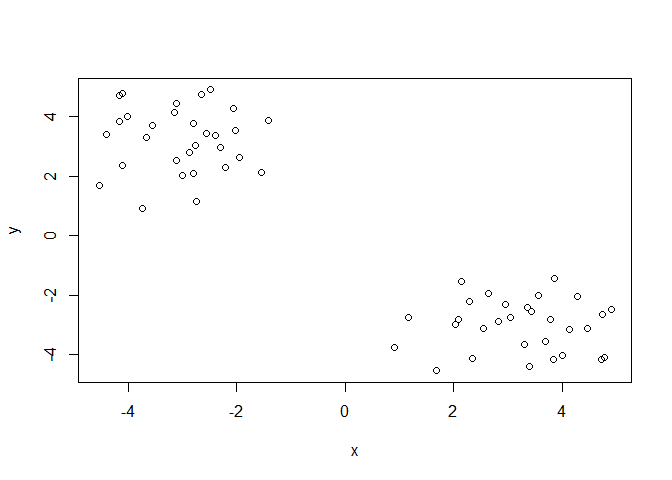
\includegraphics{Class05_R_files/figure-latex/unnamed-chunk-1-1.pdf}

\begin{Shaded}
\begin{Highlighting}[]
\KeywordTok{summary}\NormalTok{(x)}
\end{Highlighting}
\end{Shaded}

\begin{verbatim}
##     Min.  1st Qu.   Median     Mean  3rd Qu.     Max. 
## -2.84497 -0.60689  0.04362  0.03895  0.70199  3.18821
\end{verbatim}

\begin{Shaded}
\begin{Highlighting}[]
\KeywordTok{hist}\NormalTok{(x)}
\end{Highlighting}
\end{Shaded}

\includegraphics{Class05_R_files/figure-latex/unnamed-chunk-1-2.pdf}

\begin{Shaded}
\begin{Highlighting}[]
\NormalTok{weight <-}\StringTok{ }\KeywordTok{read.table}\NormalTok{(}\StringTok{"bimm143_05_rstats/weight_chart.txt"}\NormalTok{, }\DataTypeTok{header=}\OtherTok{TRUE}\NormalTok{)}
\KeywordTok{plot}\NormalTok{(weight, }\DataTypeTok{pch=}\DecValTok{15}\NormalTok{, }\DataTypeTok{cex=}\FloatTok{1.5}\NormalTok{, }\DataTypeTok{lwd=}\DecValTok{2}\NormalTok{, }\DataTypeTok{ylim=}\KeywordTok{c}\NormalTok{(}\DecValTok{2}\NormalTok{,}\DecValTok{10}\NormalTok{), }\DataTypeTok{xlab=}\StringTok{"AGE(Months)"}\NormalTok{, }
     \DataTypeTok{ylab=}\StringTok{"WEIGHT(Kg)"}\NormalTok{, }\DataTypeTok{main=}\StringTok{"Baby Weight with Age"}\NormalTok{)}
\end{Highlighting}
\end{Shaded}

\includegraphics{Class05_R_files/figure-latex/unnamed-chunk-1-3.pdf}

\begin{Shaded}
\begin{Highlighting}[]
\NormalTok{feature <-}\StringTok{ }\KeywordTok{read.table}\NormalTok{(}\StringTok{"bimm143_05_rstats/feature_counts.txt"}\NormalTok{, }\DataTypeTok{header =} \OtherTok{TRUE}\NormalTok{, }\DataTypeTok{sep =} \StringTok{"}\CharTok{\textbackslash{}t}\StringTok{"}\NormalTok{)}

\KeywordTok{par}\NormalTok{(}\DataTypeTok{mar=}\KeywordTok{c}\NormalTok{(}\DecValTok{5}\NormalTok{,}\DecValTok{12}\NormalTok{,}\DecValTok{4}\NormalTok{,}\DecValTok{3}\NormalTok{))}
\KeywordTok{barplot}\NormalTok{(feature}\OperatorTok{$}\NormalTok{Count, }\DataTypeTok{horiz=}\OtherTok{TRUE}\NormalTok{, }\DataTypeTok{xlab=}\StringTok{"feature count"}\NormalTok{, }\DataTypeTok{names.arg =}\NormalTok{ feature}\OperatorTok{$}\NormalTok{Feature, }
       \DataTypeTok{main=} \StringTok{"Feature Count"}\NormalTok{, }\DataTypeTok{las=}\DecValTok{1}\NormalTok{, }\DataTypeTok{xlim =} \KeywordTok{c}\NormalTok{(}\DecValTok{0}\NormalTok{,}\DecValTok{80000}\NormalTok{))}
\end{Highlighting}
\end{Shaded}

\includegraphics{Class05_R_files/figure-latex/unnamed-chunk-1-4.pdf}

\begin{Shaded}
\begin{Highlighting}[]
\NormalTok{phenotype <-}\StringTok{ }\KeywordTok{read.table}\NormalTok{(}\StringTok{"bimm143_05_rstats/up_down_expression.txt"}\NormalTok{, }\DataTypeTok{header=} \OtherTok{TRUE}\NormalTok{)}
\KeywordTok{table}\NormalTok{(phenotype}\OperatorTok{$}\NormalTok{State)}
\end{Highlighting}
\end{Shaded}

\begin{verbatim}
## 
##       down unchanging         up 
##         72       4997        127
\end{verbatim}

\begin{Shaded}
\begin{Highlighting}[]
\KeywordTok{palette}\NormalTok{(}\KeywordTok{c}\NormalTok{(}\StringTok{"green"}\NormalTok{, }\StringTok{"red"}\NormalTok{, }\StringTok{"blue"}\NormalTok{))}
\KeywordTok{plot}\NormalTok{(phenotype}\OperatorTok{$}\NormalTok{Condition1, phenotype}\OperatorTok{$}\NormalTok{Condition2, }\DataTypeTok{col=}\NormalTok{phenotype}\OperatorTok{$}\NormalTok{State, }
     \DataTypeTok{xlab=}\StringTok{"expresscondition 1"}\NormalTok{, }\DataTypeTok{ylab=}\StringTok{"express condition 2"}\NormalTok{)}
\end{Highlighting}
\end{Shaded}

\includegraphics{Class05_R_files/figure-latex/unnamed-chunk-1-5.pdf}

\begin{Shaded}
\begin{Highlighting}[]
\CommentTok{# Lets plot expresion vs gene regulation}
\NormalTok{meth <-}\StringTok{ }\KeywordTok{read.delim}\NormalTok{(}\StringTok{"bimm143_05_rstats/expression_methylation.txt"}\NormalTok{)}
\KeywordTok{plot}\NormalTok{(meth}\OperatorTok{$}\NormalTok{gene.meth, meth}\OperatorTok{$}\NormalTok{expression)}
\end{Highlighting}
\end{Shaded}

\includegraphics{Class05_R_files/figure-latex/unnamed-chunk-1-6.pdf}

\begin{Shaded}
\begin{Highlighting}[]
\NormalTok{dcols <-}\StringTok{ }\KeywordTok{densCols}\NormalTok{(meth}\OperatorTok{$}\NormalTok{gene.meth, meth}\OperatorTok{$}\NormalTok{expression)}

\CommentTok{# Plot changing the plot character ('pch') to a solid circle}
\KeywordTok{plot}\NormalTok{(meth}\OperatorTok{$}\NormalTok{gene.meth, meth}\OperatorTok{$}\NormalTok{expression, }\DataTypeTok{col =}\NormalTok{ dcols, }\DataTypeTok{pch =} \DecValTok{20}\NormalTok{)}
\end{Highlighting}
\end{Shaded}

\includegraphics{Class05_R_files/figure-latex/unnamed-chunk-1-7.pdf}

\begin{Shaded}
\begin{Highlighting}[]
\CommentTok{# Find the indices of genes with above 0 expresion}
\NormalTok{inds <-}\StringTok{ }\NormalTok{meth}\OperatorTok{$}\NormalTok{expression }\OperatorTok{>}\StringTok{ }\DecValTok{0}

\CommentTok{# Plot just these genes}
\KeywordTok{plot}\NormalTok{(meth}\OperatorTok{$}\NormalTok{gene.meth[inds], meth}\OperatorTok{$}\NormalTok{expression[inds])}
\end{Highlighting}
\end{Shaded}

\includegraphics{Class05_R_files/figure-latex/unnamed-chunk-1-8.pdf}

\begin{Shaded}
\begin{Highlighting}[]
\NormalTok{## Make a desnisty color vector for these genes and plot}
\NormalTok{dcols <-}\StringTok{ }\KeywordTok{densCols}\NormalTok{(meth}\OperatorTok{$}\NormalTok{gene.meth[inds], meth}\OperatorTok{$}\NormalTok{expression[inds])}

\KeywordTok{plot}\NormalTok{(meth}\OperatorTok{$}\NormalTok{gene.meth[inds], meth}\OperatorTok{$}\NormalTok{expression[inds], }\DataTypeTok{col =}\NormalTok{ dcols, }\DataTypeTok{pch =} \DecValTok{20}\NormalTok{)}
\end{Highlighting}
\end{Shaded}

\includegraphics{Class05_R_files/figure-latex/unnamed-chunk-1-9.pdf}

\begin{Shaded}
\begin{Highlighting}[]
\NormalTok{dcols.custom <-}\StringTok{ }\KeywordTok{densCols}\NormalTok{(meth}\OperatorTok{$}\NormalTok{gene.meth[inds], meth}\OperatorTok{$}\NormalTok{expression[inds],}
                         \DataTypeTok{colramp =} \KeywordTok{colorRampPalette}\NormalTok{(}\KeywordTok{c}\NormalTok{(}\StringTok{"blue2"}\NormalTok{,}
                                                      \StringTok{"green"}\NormalTok{,}
                                                      \StringTok{"orange"}\NormalTok{,}
                                                      \StringTok{"red2"}\NormalTok{)) )}

\KeywordTok{plot}\NormalTok{(meth}\OperatorTok{$}\NormalTok{gene.meth[inds], meth}\OperatorTok{$}\NormalTok{expression[inds], }
     \DataTypeTok{col =}\NormalTok{ dcols.custom, }\DataTypeTok{pch =} \DecValTok{20}\NormalTok{)}
\end{Highlighting}
\end{Shaded}

\includegraphics{Class05_R_files/figure-latex/unnamed-chunk-1-10.pdf}


\end{document}
